%%%% Proceedings format for most of ACM conferences (with the exceptions listed below) and all ICPS volumes.
\documentclass[sigconf]{acmart}
%%%% As of March 2017, [siggraph] is no longer used. Please use sigconf (above) for SIGGRAPH conferences.

%%%% Proceedings format for SIGPLAN conferences 
% \documentclass[sigplan, anonymous, review]{acmart}

%%%% Proceedings format for SIGCHI conferences
% \documentclass[sigchi, review]{acmart}

%%%% To use the SIGCHI extended abstract template, please visit
% https://www.overleaf.com/read/zzzfqvkmrfzn

\usepackage{booktabs} % For formal tables
\usepackage{graphicx}


% Copyright
%\setcopyright{none}
%\setcopyright{acmcopyright}
%\setcopyright{acmlicensed}
\setcopyright{rightsretained}
%\setcopyright{usgov}
%\setcopyright{usgovmixed}
%\setcopyright{cagov}
%\setcopyright{cagovmixed}


% DOI
\acmDOI{10.475/123_4}

% ISBN
\acmISBN{123-4567-24-567/08/06}

%Conference
\acmConference[ACMMM2017]{ACM Multimedia}{October 2017}{Mountain View, CA USA} 
\acmYear{2017}
\copyrightyear{2017}

\acmPrice{15.00}


\begin{document}
\title{Visual Analysis of Travel Route Recommendation}

\author{Dawei Chen}
\orcid{1234-5678-9012}
\affiliation{%
  \institution{Data61 \& The Australian National University}
  \streetaddress{P.O. Box 1212}
  \city{Dublin} 
  \state{Ohio} 
  \postcode{43017-6221}
}
\email{trovato@corporation.com}

\author{G.K.M. Tobin}
%\authornote{The secretary disavows any knowledge of this author's actions.}
\affiliation{%
  \institution{Institute for Clarity in Documentation}
  \streetaddress{P.O. Box 1212}
  \city{Dublin} 
  \state{Ohio} 
  \postcode{43017-6221}
}
\email{webmaster@marysville-ohio.com}

\author{Lars Th{\o}rv{\"a}ld}
\affiliation{%
  \institution{The Th{\o}rv{\"a}ld Group}
  \streetaddress{1 Th{\o}rv{\"a}ld Circle}
  \city{Hekla} 
  \country{Iceland}}
\email{larst@affiliation.org}

% The default list of authors is too long for headers}
\renewcommand{\shortauthors}{D. Chen et al.}


\begin{abstract}
We propose a novel travel route visualisation tool. 
\end{abstract}

%
% The code below should be generated by the tool at
% http://dl.acm.org/ccs.cfm
% Please copy and paste the code instead of the example below. 
%
\begin{CCSXML}
<ccs2012>
 <concept>
  <concept_id>10010520.10010553.10010562</concept_id>
  <concept_desc>Computer systems organization~Embedded systems</concept_desc>
  <concept_significance>500</concept_significance>
 </concept>
 <concept>
  <concept_id>10010520.10010575.10010755</concept_id>
  <concept_desc>Computer systems organization~Redundancy</concept_desc>
  <concept_significance>300</concept_significance>
 </concept>
 <concept>
  <concept_id>10010520.10010553.10010554</concept_id>
  <concept_desc>Computer systems organization~Robotics</concept_desc>
  <concept_significance>100</concept_significance>
 </concept>
 <concept>
  <concept_id>10003033.10003083.10003095</concept_id>
  <concept_desc>Networks~Network reliability</concept_desc>
  <concept_significance>100</concept_significance>
 </concept>
</ccs2012>  
\end{CCSXML}

\ccsdesc[500]{Computer systems organization~Embedded systems}
\ccsdesc[300]{Computer systems organization~Redundancy}
\ccsdesc{Computer systems organization~Robotics}
\ccsdesc[100]{Networks~Network reliability}

% We no longer use \terms command
%\terms{Theory}

\keywords{ACM proceedings, \LaTeX, text tagging}

% Used in some conference proceedings e.g. sigplan and sigchi
 \begin{teaserfigure}
 \centering
   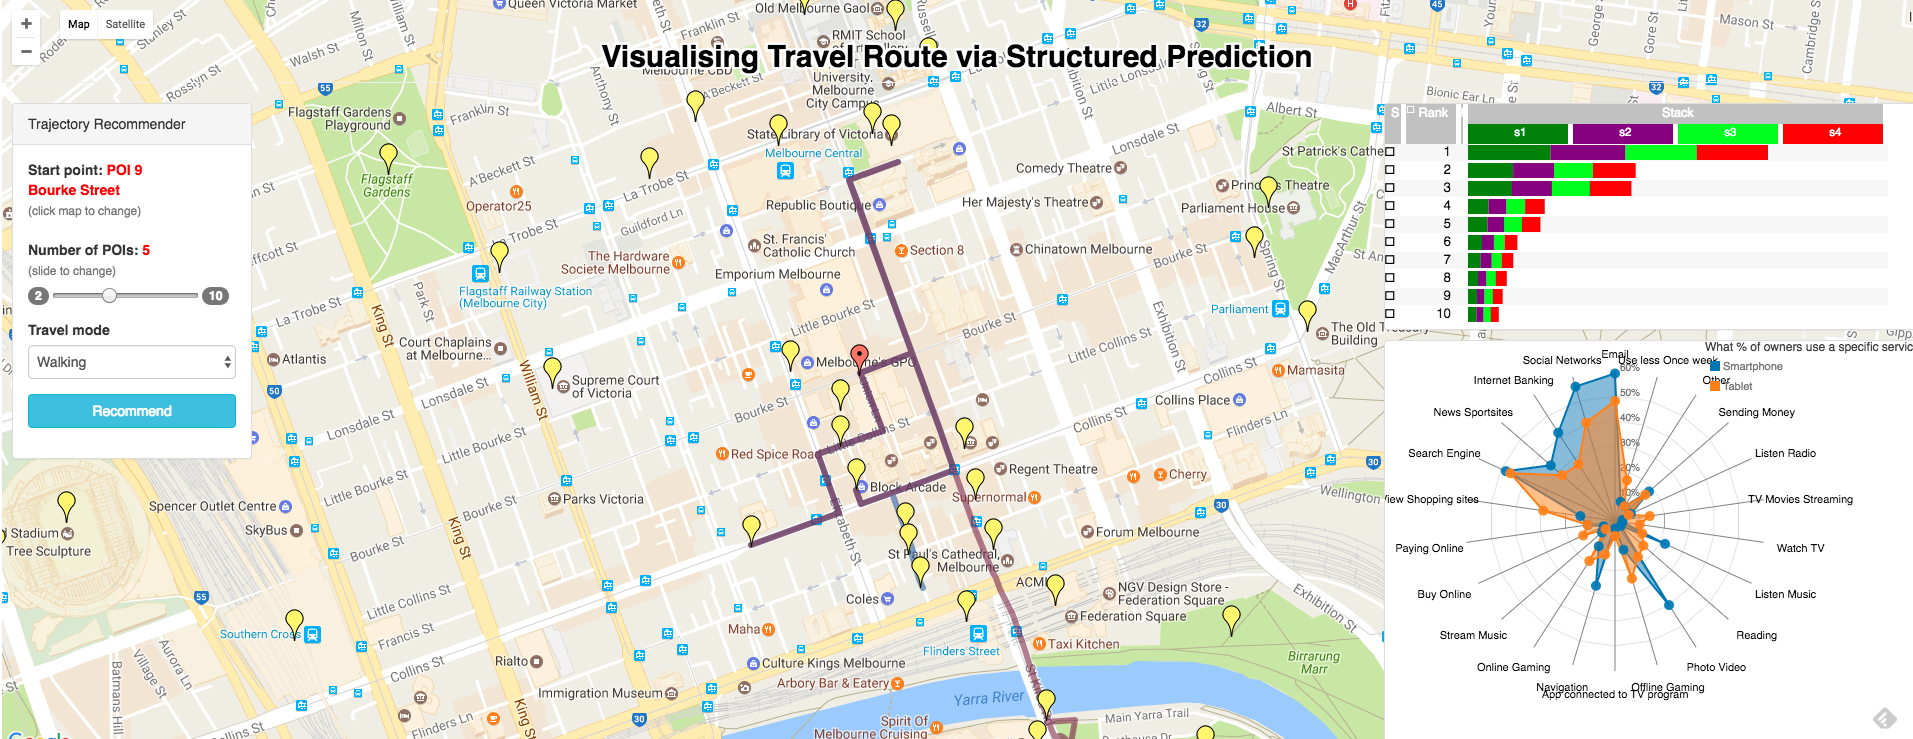
\includegraphics[width=0.8\textwidth]{figure/sample_map.png}
   \caption{Travel route recommendation visualisation system. Given a starting POI and a number of POI to be visited, the system suggests a set of routes from a history of previous tourists.}
   \label{fig:overview}
 \end{teaserfigure}

\maketitle


\section{Introduction}
%background
Sequence ranking has emerged as an important tool for solving diverse problems such as travel route and music playlist recommendations. Unlike the classical ranking algorithm where each item considers independently, the sequence ranking algorithm requires modelling a structure between items and suggests a set of items as a whole. For example, let us consider recommending a trajectory of points of interest (POI) in a city to a visitor. If the classical ranking algorithm learns a user's preference for each individual location while ignores the distances between them, the algorithm may create a long trajectory, which should be shorter in optimal routeing. Several sequence ranking algorithms are proposed to solve the problem and achieve relative success to compare with the classical algorithms. An important challenge remaining is to construct a visualisation of the recommendation system so that a user can analyse the suggested sequences and plan a better trip based on the interaction with the system.

%approach
In this paper, we tackle the problem of sequence visualisation, especially, in the context of a travel route recommendation. We first define and formulate the sequence ranking algorithm as a structured recommendation problem, and then we develop a novel visualisation engine that efficiently displays multiple suggested routes and helps users understand the rational behind the recommendations. Specifically, we formulate a travel route as a sequence of points-of-interest (POIs)...

\section{Structured Prediction}
% don't need very details of the algorithm
% need problem definition
% copied from nips paper
Travel route recommendation problems involve a set of POIs in a city. Given a trajectory query $\mathbf{x} = (s, l)$, comprising a start POI $s$ and trip length $l$, i.e. the number of POIs to be visited during the trip including $s$, the goal is to suggest one or more sequences of POIs that maximise some notion of utility.

We first cast the travel recommendation as a structured prediction problem, which allows us to leverage the well-studied literature of structured SVMs (SSVM)~\cite{tsochantaridis2005large,joachims2009predicting}. There are two obstacles to prevent us applying the SSVM directly to the sequence recommendation problem; first, there would be multiple possible routes among a set of POIs, second, a naive application of SSVM would generate repeating sequence in the prediction time. 
To eliminate possible loop in a prediction time, we adopt serial list Viterbi~\cite{seshadri1994list,nill1995list} algorithm.
We finally trained our model on the trajectory data extracted from Flickr photos~\cite{chen2016learning}.

From a visualisation perspective, an important advantage of the SSVM is the explicit representation of feature score in its final decision process. Especially, in our case, we can disassemble the final score of a route into feature scores of each POI and each transition between two adjacency POIs. We hand-crafted POI features such as the category, popularity, average spending time of previous tourists, etc, and also crafted transition features such as the distance between two POIs, .

\section{Visualisation}
%what are the features we want to emphasis?
%make a bullet list of something like that
Our goal is to design an interactive system where a user 
The Figure \ref{fig:overview}
Break total score into individual feature score, represent using stacked bar graph.

Comparison between two POIs in a single trajectory.
Further comparison of POIs within a single trajectory, we use radar chart to show the score of each feature.

We further provide a tool to analyse an internal variation between multiple POIs in a single route. 
Figure \ref{fig:radar} shows the feature scores of two POIs in a single route via a radar plot. 

Stacked bar plot \cite{gratzl2013lineup}


\begin{figure}[t!]
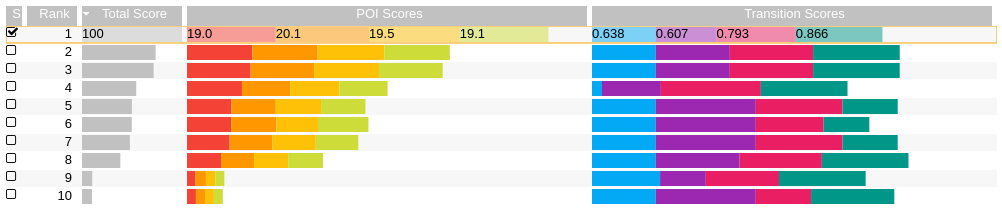
\includegraphics[width=0.9\linewidth]{figure/sample_stack.png}
\caption{Visualisation of feature scores for each trajectory. From top to bottom, we represent top 10 recommended routes with their scores where each score is further decomposed into multiple features.}
\end{figure}

\begin{figure}[t!]
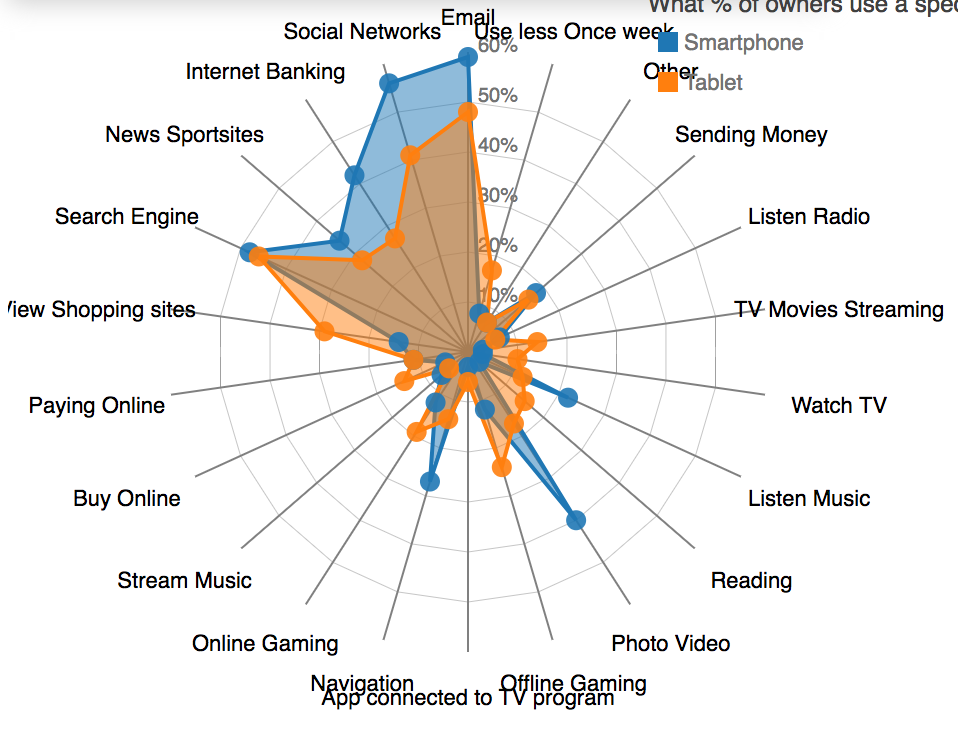
\includegraphics[width=0.9\linewidth]{figure/sample_radar.png}
\caption{Visualisation of feature score for each POI within a single route.}
\label{fig:radar}
\end{figure}


\section{Conclusion}
%summary


\bibliographystyle{ACM-Reference-Format}
\bibliography{sigproc} 

\end{document}
